\documentclass[letterpaper,11pt,twoside]{report}
\usepackage{epsfig,epstopdf}
\usepackage{float,captdef,multicol,fancybox}
\usepackage[a4paper,pdftex]{geometry}
\usepackage[utf8]{inputenc}
\setlength{\oddsidemargin}{5mm}			
\setlength{\evensidemargin}{5mm}

\usepackage[spanish,activeacute]{babel}
\usepackage[protrusion=true,expansion=true]{microtype}	
\usepackage{amsmath,amsfonts,amsthm,amssymb,dsfont}
\usepackage{graphicx,wrapfig,lipsum}
\usepackage[section]{placeins}
\usepackage{float}
\usepackage{multicol}
\providecommand{\abs}[1]{\lvert#1\rvert}
\providecommand{\norm}[1]{\lVert#1\rVert}
%\usepackage[right=4.5cm,left=2cm,top=2cm,bottom=2.0cm,headsep=0.7cm,footskip=1.0cm]{geometry}


\usepackage{fancyhdr}
\fancyhf{} % clear all header and footers
\renewcommand{\headrulewidth}{0pt} % remove the header rule
\fancyfoot[RE,LO]{\thepage} % Left side on Even pages; Right side on Odd pages
\pagestyle{fancy}
\fancypagestyle{plain}{%
	\fancyhf{}%
	\renewcommand{\headrulewidth}{0pt}%
	\fancyhf[lef,rof]{\thepage}%
}



\newcommand{\HRule}[1]{\rule{\linewidth}{#1}} 	

\makeatletter							
\def\printtitle{						
	{\centering \@title\par}}
\makeatother									

\makeatletter							
\def\printauthor{				
	{\centering \large \@author}}				
\makeatother							

\title{	\normalsize \textsc{} 	
	\\[2.0cm]							
	\HRule{1pt} \\						
	\LARGE \textbf{\uppercase{Geometr\'ia Diferencial: \\ Geometr\'ia Gaussiana}}	
	\HRule{1pt} \\ [0.5cm]		
	\normalsize \today}

\author{Ricardo Stuardo T.}

\begin{document}
	
	\thispagestyle{empty}	
	

\printtitle					
\vfill
\begin{flushright}
	\printauthor
\end{flushright}

\newpage
	\thispagestyle{empty}
	\ \\

\newpage

	\thispagestyle{empty}
	\pagenumbering{gobble}
	\tableofcontents

\newpage
	\thispagestyle{empty}
	\ \\


\newpage

	\thispagestyle{empty}
	\pagenumbering{gobble}

	\bigskip \
	\bigskip \
	\bigskip \
	\bigskip \
	\bigskip \
	\bigskip \	
	\bigskip \
	\bigskip \
	\bigskip \	
	\bigskip \
	\bigskip \
	\bigskip \
	\bigskip \
	\bigskip \
	\bigskip \	
	\bigskip \
	\bigskip \
	\bigskip \
	
	\begin{center}
		\emph{\textquotedblleft Pure mathematics is, in its way, the poetry of logical ideas."}
	\end{center}
	
	\begin{flushright}
		Albert Einstein.
	\end{flushright}

\newpage
	\thispagestyle{empty}
	\ \\

\newpage
	\pagenumbering{arabic}
	\setcounter{page}{1}

\chapter{Curvas}
	
\section{Concepto de Curva}

Una curva es un mapeo diferenciable desde un conjunto abierto $I$ de $\mathbb{R}$ a una regi\'on $\mathcal{C}$ de $\mathbb{R}^{3}$:
	 \begin{align*}
		M: I \subset \mathbb{R} &\longrightarrow \mathcal{C} \subset \mathbb{R}^{3} \\
		   t &\longmapsto x^{i} = x^{i} (t)  \ \ \ \ , i = 1,2,3
	 \end{align*}

\begin{figure}[h!]
	\begin{center}
		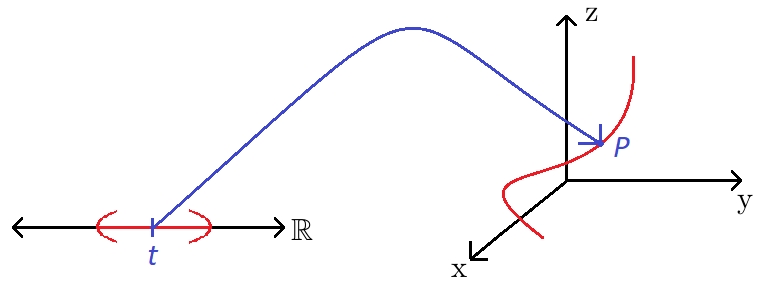
\includegraphics[width=10cm]{idea_curva.png}
	\end{center}
	\label{figc1}
	\caption{Idea de Curvas}
\end{figure}

El punto $t \in \mathbb{R}$ es mapeado en el punto $P \in \mathcal{C}$. La imagen de $I$ de $\mathbb{R}$ es la linea roja mostrada en 
$\mathcal{C}$, y la linea azul representa el mapeo de $I$ en $\mathcal{C}$. \\

As\'i tenemos que uno asocia cada pundo de $\mathbb{R}$, con un punto en $\mathcal{C}$, el cual es llamado el punto imagen de 
$t$, El conjunto de todos los puntos imagenes es la noci\'on ordinaria de curva. Esta definici\'on asocia a cada punto de $\mathcal{C}$ 
un valor de $t$, es decir, tenemos una curva parametrizada con un par\'ametro $t$:
	\begin{equation*}
		\mathcal{C} = \left\{ \textbf{x}(t) \in \mathbb{R}^{3}: t \in I  \right\}
	\end{equation*}

Donde se dice que ($\textbf{x},I$) es una representaci\'on param\'etrica de $\mathcal{C}$, y a $t$ se le llama \textit{par\'ametro} de la 
curva . \\

Cuando pedimos que sea un mapeo diferenciable, queremos decir que las coordenadas de los puntos imagenes ( $ x^{i} = x^{i}(t)$ ) son 
funciones diferenciables. As\'i una curva $\mathcal{C}$ queda descrita por las ecuaciones:
	\begin{equation*}
		x^{i} = x^{i}(t)
	\end{equation*}
	
o bien
	\begin{equation*}
		\textbf{x} = \textbf{x}(t)
	\end{equation*}

\subsection{Parametrizaci\'on Regular}

Sea una funci\'on vectorial: 
	\begin{equation*}
		x^{i} = x^{i}(t) \ \ \ \ , t \in I  
	\end{equation*}

Se dice que es una representaci\'on param\'etrica regular de parametro $t$ si se satisfacen las siguientes propiedades:
	\begin{itemize}
		\item	$x^{i}(t)$ es de clase $C^{1}$ en $I$.
		\item	$\frac{dx^{i}}{dt} = x'^{i} \neq 0$ para todo $t$ en $I$ (que es equivalente a $ \left| \textbf{x}'\right| \neq 0$ ).
	\end{itemize}

Una representaci\'on param\'etrica regular, puede poseer puntos multiples, es decir, pueden existir $t_{1}$ y $t_{2}$, 
tal que $t_{1} \neq t_{2}$ para los cuales $x^{i}(t_{1}) = x^{i}(t_{2})$. Sin embargo, localmente, esto no ocurre.

\subsection{Curvas Regulares}

Una funci\'on num\'erica $t = t(\theta)$ en un intervalo $I_{\theta}$ es un cambio admisible de par\'ametro si:
	\begin{itemize}
		\item	$t = t(\theta)$ es de clase $C^{1}$ en $I_{theta}$.
		\item	$\frac{dt}{d\theta} \neq 0$ para todo $\theta$ en $I_{\theta}$.
	\end{itemize}

\textbf{Teorema}: Si $t = t(\theta)$ representa un cambio admisible de par\'ametro en $I_{\theta}$, entonces :
	\begin{itemize}
		\item	$t = t(\theta)$ es una aplicaci\'on inyectiva de $I_{theta}$ en un intervalo $I_{t} = t(I_{\theta})$
		\item	La funci\'on inversa $\theta = \theta(t)$ es a su vez un cambio admisible de par\'ametro en $I_{t}$
	\end{itemize}

Notemos que, $x^{i} = x^{i}(t)$ determina unicamente una curva $\mathcal{C}$ que consta de todas las representaciones que se 
relacionan con ella a partir de un cambio admisible de par\'ametro. Sin embargo, puede ocurrir que la parametrizaci\'on $x^{i} = x^{i}(t)$  
tenga una propiedad que no sea neesariamente una propiedad de la curva. Por otro lado, las propiedades de la curva deben ser com\'unes a 
todas las parametrizaciones, es decir, las propiedades de la curva son \textit{independientes del par\'ametro}. \\

Un ejemplo de esto son las llamadas curvas simples, que corresponde a una curva regular sin puntos multiples.

\subsection{Longitud de Arco}

Sea $I = (a,b) \in \mathbb{R}$ un intervalo abierto, y sea $\mathcal{C}: I \longrightarrow \mathbb{R}^{3}$ una curva parametrizada con 
par\'ametro $t$ ( $x^{i} = x^{i}(t)$ ). La longitud de arco de la curva desde $\textbf{x}(t_{0})$ a $\textbf{x}(t)$ es:
	\begin{equation*}
		s(t) = \int^{t}_{t_{0}} \left| \frac{d\textbf{x}}{dt'}\right| dt' =  \int^{t}_{t_{0}} \sqrt{ \left( \frac{dx^{1}}{dt'} \right)^{2} + \left( \frac{dx^{2}}{dt'} \right)^{2} + \left( \frac{dx^{3}}{dt'} \right)^{2}} dt'
	\end{equation*}
	
\subsection{Parametrizaci\'on Natural}

Del teorema fundamenteal del c\'alculo, sabemos que:
	\begin{equation*}
		\frac{ds}{dt} = \frac{d}{dt} \int^{t}_{t_{0}} \left| \frac{d\textbf{x}}{dt'}\right| dt' = \left| \frac{d\textbf{x}}{dt}\right|
	\end{equation*}
	
Donde $x^{i} = x^{i}(t)$ es una curva parametrizada con par\'ametro $t$. Esta curva puede ser parametrizada con par\'ametro $s$ si y solo si 
$s = s(t)$ es un cambio admisible de par\'ametro en $I$. De acuerdo con el teorema reci\'en planteado, $s = s(t)$ ser\'a un cambio admisible de 
par\'ametro en $I$ si:
	\begin{itemize}
		\item	$s = s(t)$ es de clase $C^{1}$ en $I$.
		\item	$\frac{ds}{dt} \neq 0$ para todo $t$ en $I$.
	\end{itemize}

Ya que $x^{i} = x^{i}(t)$ es una parametrizaci\'on regular, tenemos que $\left| \frac{d\textbf{x}}{dt}\right| \neq 0$ y de esto vemos que 
$\frac{ds}{dt} \neq 0$. Luego, si $s(t)$ es de clase $C^{m}$ en $I$, tenemos que $s = s(t)$ es un cambio admisible de par\'ametro, por lo que, 
\textbf{la longitud de arco $s$ puede ser usada como par\'ametro a lo largo de la curva}. A $s$ se le llama \textit{par\'ametro natural}, y a 
$x^{i} = x^{i}(s)$ se le llama \textit{parametrizaci\'on natural}. \\
	
\textbf{Ejemplo:} Encontremos el par\'ametro natural, y reparametrizemos la siguiente curva:
	\begin{equation*}
		\textbf{x} = (e^{t} \cos(t))\hat{i} + (e^{t} \sin(t))\hat{j} + e^{t}\hat{k} \ \ \ \ \ \ \ , \text{con}  -\infty < t < \infty
	\end{equation*}

De donde:
	\begin{align*}
		x^{1} &= e^{t} \cos(t) \\
		x^{2} &= e^{t} \sin(t) \\
		x^{3} &= e^{t}
	\end{align*}

Veamos que:
	\begin{align*}
		\frac{dx^{1}}{dt} &= \frac{d}{dt}\left( e^{t} \cos(t) \right) = e^{t} \cos(t) - e^{t}\sin(t) \\
		\frac{dx^{2}}{dt} &= \frac{d}{dt}\left( e^{t} \sin(t) \right) = e^{t} \sin(t) + e^{t}\cos(t) \\
		\frac{dx^{3}}{dt} &= \frac{d}{dt}\left( e^{t} \right) = e^{t} 
	\end{align*}

Por lo que:
	\begin{align*}
		\left| \frac{d\textbf{x}}{dt}\right| &= \sqrt{ \left( \frac{dx^{1}}{dt} \right)^{2} 
													 + \left( \frac{dx^{2}}{dt} \right)^{2} 
													 + \left( \frac{dx^{3}}{dt} \right)^{2}} \\
											 &= \sqrt{ \left( e^{t} \cos(t) - e^{t}\sin(t) \right)^{2} 
											         + \left( e^{t} \sin(t) + e^{t}\cos(t) \right)^{2} 
											         + \left( e^{t}  \right)^{2} } \\
											 &= \sqrt{ e^{2t} \cos^{2}(t) -2e^{2t}\cos(t)\sin(t) + e^{2t}\sin^{2}(t)  
											         +  e^{2t}\sin^{2}(t) +2e^{2t}\cos(t)\sin(t) + e^{2t}\cos^{2}(t)
											         +  e^{2t} } \\
											 &= \sqrt{ 3 e^{2t} } \\
											 &= \sqrt{3} e^{t} 
	\end{align*}

Luego, para encontrar $s$ integramos $\left| \frac{d\textbf{x}}{dt}\right|$ entre $t_{0}$ y $t$:
	\begin{align*}
		s &= \int^{t}_{t_{0}} \left| \frac{d\textbf{x}}{dt'}\right| dt' \\
		  &= \int^{t}_{t_{0}} \sqrt{3} e^{t'} dt' \\
		  &= \sqrt{3} e^{t} \big|^{t}_{t_{0}} \\
		  &= \sqrt{3} \left( e^{t} - e^{t_{0}} \right)
	\end{align*}

Despejando $t$, obtenemos:
	\begin{equation*}
		t = \ln \left(\frac{s}{\sqrt{3}}+e^{t_{0}} \right) \ \ \ \ \ \ \ , \text{con} \ \  -\sqrt{3}e^{t_{0}} < s < \infty
	\end{equation*}

Introduciendo $s$ como par\'ametro obtenemos:
	\begin{align*}
		x^{1} &= e^{ \left( \frac{s}{\sqrt{3}}+e^{t_{0}} \right) } \cos \left( \ln \left( \frac{s}{\sqrt{3}}+e^{t_{0}} \right) \right) \\
		x^{2} &= ( e^{ \left( \frac{s}{\sqrt{3}}+e^{t_{0}} \right)}	\sin\left(\ln \left(\frac{s}{\sqrt{3}}+e^{t_{0}} \right) \right)  \\
		x^{3} &= e^{ \left(\frac{s}{\sqrt{3}}+e^{t_{0}} \right) }
	\end{align*}

Del ejemplo, vemos que, pareciera que el par\'ametro depende del punto del cual integremos el la longitud de la curva ($t_{0}$), lo que nos 
hace pensar, ¿Habr\'a m\'as de un par\'ametro natural para una misma curva?. La respuesta esta en el siguiente teorema:\\

\textbf{Teorema}: Si $x^{i} = x^{i}(s)$ es una representaci\'on natural de $\mathcal{C}$, entonces: 
	\begin{itemize}
		\item Si $x^{i} = x^{*i}(s^{*})$ es cualquier otro tipo de representaci\'on natural de $\mathcal{C}$, entonces: $s = \pm s^{*} + \text{constante}$.
	\end{itemize}
	
Volviendo al ejemplo anterior, teniamos que el parº'ametro (o la parametrizaci\'on) dependian de $e^{t_{0}} = c$ con $c$ una constante 
positiva, de acuerdo al teorema anterior, esto es completamente normal, ya que depende en forma aditiva de esta constante, luego, podemos definir 
un $s^{*} = s - c' $ para eliminar la constante aditiva.  \\

Desde ahora en adelante, usaremos la siguente notaci\'on:
	\begin{equation*}
		\dot{\textbf{x}} = \frac{d\textbf{x}}{ds} \ \  , \ \ \ddot{\textbf{x}} = \frac{d^{2}\textbf{x}}{ds^{2}}\ \ , \ \ 
		\textbf{x}' = \frac{d\textbf{x}}{dt}\ \ , \ \ \textbf{x}'' = \frac{d^{2}\textbf{x}}{dt^{2}}
	\end{equation*}
	
\section{Curvatura y Torsi\'on}

\subsection{Vector Unitario Tangente}

\section{Teor\'ia de las Curvas}

\chapter{Superficies}

\section{Concepto de Superficie}

\section{Formas Fundamentales}

\subsection{Primera Forma Fundamental}

\subsection{Segunda Forma Fundamental}

\section{Teor\'ia de Superfices}

\section{Geometria Intr\'inseca}



\end{document}
